%{{{ preamble
% Note: The order of some of these packages are important.
% fleqn left alligns all equations. Using settings from uiophd.cls.
\documentclass[altfont, fleqn]{uiophd}
\usepackage[T1]{fontenc}
\usepackage[utf8]{inputenc}
\usepackage[usenames,dvipsnames,svgnames]{xcolor}			
% Rebinds commands safer than using \let\mycref\cref.
\usepackage{letltxmacro}
% Can change properties of sections, such as color. 
\usepackage{titlesec}		
% Adds customizable headers and footers. 
\usepackage{fancyhdr}		
% Adds small toc lists. 
\usepackage{titletoc}		
\usepackage{hyperref}
\usepackage{graphicx}
% Essential math package.
\usepackage{amsmath}		
% \abs and \norm.
\usepackage{commath}		
% Do not know.
\usepackage{textcomp}
% SI units package.
\usepackage[redefsymbols=false]{siunitx}		
% Some extra signs and other fonts.
\usepackage{bm,upgreek} 
\usepackage{appendix}
\usepackage[
	backend=biber,
	style=numeric,
	doi=false,
	% isbn=false, 
	maxcitenames=2,
]{biblatex}
% Have to import this at the end for this to work somehow.
\usepackage{cleveref}		
\usepackage{multicol}
% Commands that help placing figures side by side.
\usepackage{subcaption}

% Glossary packages.
% \usepackage[nopostdot,toc]{glossaries}
% % Enables multi column glossary.
% \usepackage{glossary-mcols}
% % Necessary for the glossaries package.
% \makeglossaries

\addbibresource{master.bib}

% Remove certain fields from appearing in the bibliography.
\AtEveryBibitem{\clearfield{month}}
\AtEveryBibitem{\clearfield{day}}
\AtEveryBibitem{\clearfield{note}}
\AtEveryCitekey{\clearfield{month}}
\AtEveryBibitem{%
    \ifentrytype{misc}
    {%
    }%
    {%
        \clearfield{url}
        \clearfield{urldate}
    }%
}

% Use ampersand "&" instead of "and". 
\renewcommand*{\finalnamedelim}{%
    \ifnumgreater{\value{liststop}}{2}{\finalandcomma}{}%
    \addspace\&\space%
}
% Paper properties. 
\pagestyle{fancy}
% Removes the header bar and text.
\renewcommand{\headrulewidth}{0pt}
\fancyhead{}
% Custom colors.
\definecolor{viridis_01}{rgb}{0.267004, 0.048740, 0.329415}
\definecolor{viridis_02}{rgb}{0.190631, 0.407061, 0.556089}
\definecolor{viridis_03}{rgb}{0.208030, 0.718701, 0.472873}
\definecolor{viridis_04}{rgb}{0.993248, 0.906157, 0.143936}
% Change section formatting.
\titleformat{\section}
    {\color{viridis_02}\Large\bfseries}
    {\color{viridis_02}\thesection}{1em}{} 		
% Change section formatting.
\titleformat{\subsection}
    {\color{viridis_02}\large\bfseries}	
    {\color{viridis_02}\thesubsection}{1em}{}
% Change section formatting.
\titleformat{\chapter}[hang] 				
    {\bfseries\Huge} 	
    {\color{viridis_01}\thechapter\hspace{20pt}\rule[-3pt]{2pt}{23pt}\hspace{10pt}}
    {0.5ex} 			
    {\color{viridis_01}} 	
    [
        % This will be applied after each chapter?
        %\small
        %\startcontents
        %\printcontents{}{1}{\setcounter{tocdepth}{1}}
    ]		
% Change the color of every citation.
\AtEveryCite{\color{viridis_03}}
% Hyperlink colors. 
% Empty color disables coloring.
\hypersetup{
	colorlinks=true,
	citecolor=viridis_03,
	filecolor=black,
	linkcolor={},
	urlcolor=black
}

% Glossary settings commented out:
% % Change the color of the glossary commands \gls and \Gls.
% \LetLtxMacro{\mygls}{\gls}
% \renewcommand{\gls}[1]{{\color{viridis_03}\mygls{#1}} }
% \LetLtxMacro{\myGls}{\Gls}
% \renewcommand{\Gls}[1]{{\color{viridis_03}\myGls{#1}} }
% % Include the glossary file. 
% \newglossaryentry{regspike}{
    name={regular spiking},
    description={Often compared to fast spiking}
}

\newglossaryentry{fastspike}{
    name={fast spiking},
    description={A short durtion extracelluar spike}
}


% Change the emph command.
\DeclareTextFontCommand{\emph}{\color{viridis_03}}
% Change color of clever ref.
\AtBeginDocument{
    \LetLtxMacro{\mycref}{\cref}
	\renewcommand{\cref}[1]{{\color{viridis_03}\mycref{#1}} }
}
%}}} end of preamble
\begin{document}
% Overview {{{ %
\chapter*{Overview}

Abstract (1/10):
\newline
Summary of the summary. A short introduction with results stated clearly.
\newline

Introduction (1/10):
\newline
Introduce the topic, the problem and how the problem is being solved. 
The target audience are other master students. 
% Keywords: Action potential shape, cell classification, electrodes.
\newline 

Theory:
\begin{itemize}
    \setlength\itemsep{0pt}
    \item Basic information about neurons and the cell membrane. (7/10)
    \item Basic information about different types of neurons, how they serve
        different purposes and have different functions. (0/10)
    \item Turning the neuron into a electronic circuit, explaining ion pumps and 
        channels. (5/10)
    \item Explanation of action potentials and the generation of
        action potentials with a the hudgekin and huxley model. (1/10)
    \item Explanation of the principle of compartmental models with diagrams.
        There are many kinds. Not too long. (0/10)
    \item Explanation of electrodes, how they are used,
        what they measure, how tetrodes work. (1/10)
    \item Mentioning that neurons measured from the same electrode must
        be seperated. Cocktail party problem, source seperation. (0/10)
    \item Explanation of extracellular potential, the physics behind the
        problem, current sum to zero, how it can be calculated, etc.(4/10)
    \item Discussion of the difference between intracellular and extracellular 
        spike shape. Some say the extracellular spike is the derivative. (0/10)
    \item Explanation of Neuron and LFPy. How they work, the principle 
        behind them, what they are intended to calculate. (2/10)
    \item Explanation of the current state of cell classification.
        Why is it important, how is it done. Mentioning most influential 
        work from early to current work. (0/10)
    \item Explanation of the Blue Brain cell database, how it was made, 
        why is it useful, what were the focus of the models, models are public. (0/10)
\end{itemize}
\noindent 
Note to self, mention the most influential work that has been done on all
topics mentioned in the theory. I should show I know all the basic 
important work that has been done in these fields. 
\newline

Methods
\newline
Everything here is work which I have done myself. Show what I have done, make sure
it understood as a lot.
\begin{itemize}
    \item Explanation of the basis of differentiating spikes, how does
        one measure how spikes are different. Meantion spike width and 
        ampltiude. (0/10)
    \item Explain different definitions of spike width and amplitude measurements. (1/10)
    \item Detailed explanation about the simulation environment. 
        What does LFPyUtil solve and how does it solve it. (3/10)
    \item Showing a minimum working example of LFPyUtil, show what it makes easier. (0/10)
    \item Detailed explanation of each simulation, what are the parameters. (3/10)
    \item How did I use the BlueBrain models, which models are used, why are they used. (0/10)
\end{itemize}

Results:
\newline
State the results in such a way they clearly show what I want to show, but
does not "jump to conclusions". State the results without bias.
Include figures with text, at a glance the figures will be read seen and read
first. 
\begin{itemize}
    \item Detailed explanation of the replication of Pettersen and Einevoll, show 
        that the simulation environment can be trusted. (6/10)
    \item Explain any deviations from Pettersen and Einevoll in the replication. (5/10)
    \item Create a conclusion of the results from Pettersen and Einevoll. (0/10)
    \item Show which definition is best for differentiating spikes from different
        kinds of neurons. (0/10)
    \item Show that interneurons and pyramidal neurons can be classified. (0/10)
    \item Explain why spikes look differnt, what are the physical processes that 
        does this? (0/10)
\end{itemize}

Discussion:
\newline
The discussion is important, make it of high quality and maybe long. 
\begin{itemize}
    \item Using spike width have already been used for differentiate neurons, 
        show how current results backs up this statement. (0/10)
    \item Research has shown that thin spikes can also come from measuring near
        axons of pyramidal cells. (0/10)
    \item Argue that the models are relateable to real spikes. (0/10)
    \item The analysis framework can be used for future cell models. (0/10)
\end{itemize}

Note to self, when trying to explain a method first show the problem clearly
then propose the solution to the problem. Engage the reader by showing the 
problem in such a way they can become curious for a solution. 


% }}} Overview %
%{{{ Abstract
\chapter*{Abstract}
\noindent
The physical processes that creates electrical signals in neurons are well understood, 
but how the signals are processed into actions and thoughts has yet to 
receive a scientifically robust answer
Cell type classification is of high importance because the function of different 
neurons is still largely a mystery. 
%}}} end of Abstract
%{{{ Table of Contents
\setcounter{tocdepth}{1}
\startcontents
\tableofcontents
%}}} end of Table of Contents
%{{{ Introduction
\chapter{Introduction}

Since 
the conception of neuroscience the neurons function have been studied on many levels
from the properties of the cell membrane to clustered networks of neurons.


There are several types of neurons 
and it was early noticed that different kind of neurons gave different
types of signals. 

This was of much interest because 


% The problem
% While doing single cell recordings the only information
% about the neuron that is avaiable is the electric signal from the neuron.
Modern types of 
classification uses genotype?, the structure of the neuron and the 
electric signal.

It is useful to seperate interneurons from pyramidal neurons as
pyramidal neurons are excitatory and interneurons are inhibitory. 

Is it possible to seperate interneurons from pyramidal neurons soly
based on the shape of the action potental. 

Knowing the neuron type is important for research. 
While doing single cell recordings on alive subjects the researchers are
recording in the dark. 
The electrodes only pick up on electrical signals from the brain, 
so the researcher does not know exactly what they cell they are recording. 

Surely the different types of neurons are specialized at certain functions

In this article we show that interneurons can be seperated from pyramidal
neurons based on data and models from the Blue Brain project. 
The program makes an easy way to do the same analysis
on future models as long as the models can be loaded with LFPy.


%}}} end of Introduction
%{{{ Theory
\chapter{Theory}
% NOTE: 
% The physical processes in and around neurons are well understood in comparison
% to the function they serve. 
% The basic function of a neuron is to receive and send 
% action potentials, 
% but what exact information is being transmitted or how 
% it is processed into thoughts does still not have a conclusive answer.

\vspace{1em} 
\startcontents
\printcontents{}{1}{\setcounter{tocdepth}{2}}
  
%{{{ The Neuron
\section{The Neuron}
\begin{figure}[h]
    \centering
    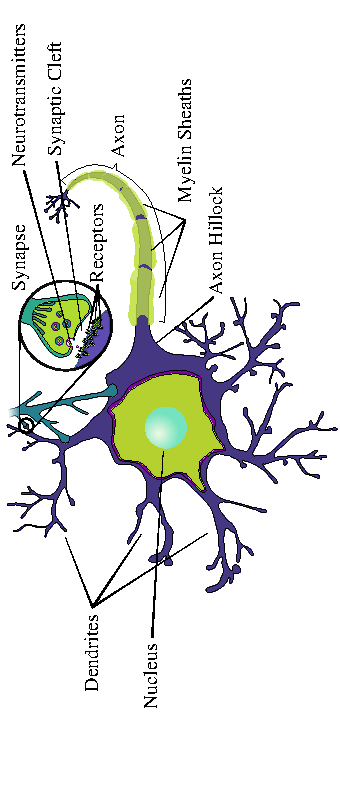
\includegraphics[angle=-90,width=1.0\textwidth]{images/2_1/neuron_structure.pdf}
    \caption{Stuff about this neuron.}
    \label{fig:2_1_neuron}
\end{figure}
\noindent
{Neurons} 
are electrically excitiable cells
that are a fundamental part of all brain functions.
Other names include {nerve cells}, {neurone} or more 
colloquially {brain cells}.
Neurons form in big networks 
which process information,
and in the human brain there is an estimated $10^{11}$ neurons.

Special proteins in the cell membrane enables the neuron to
fire action potentials when it is electrically excited. 
These action potentials are sharp voltage changes that propagates through
the full structure of the neuron. 
The same properties that makes the neuron able to fire makes 
the action potential {regenerative}, meaning it will propagate
without decay.

The body of the neuron, the {soma}, has {dendrites} and 
the {axon} attached to it. 
The dendrites and the axon are very thin branching structures 
with a width usually in the order of \SI{1}{\micro\metre}. 
While neurons often have many dendrites directly attached to the soma
there is only one axon attached through the \emph{axon hillock}.
The axon can branch several times before it ends and 
usually connects to the dendrites of other neurons via synapes.

The synapes are electrically sensitive which allows information
to pass between neurons. 
Though the majority of all synapes are axo-dendritic 
(axon to dendrite),
other junctions are also possible.
Other junctions include but are not limited to,
dendrite to dendrite, 
axon to axon and 
axon to blood vessel. 
When an action potential reaches a synapse it will activate
the synapse and pass information to the connect neuron. 
The information that is passed along depends on the type of synapse,
and if it is of a chemical or electrical type.

% NOTE: Topic to mention:
% Neuron cell types, pyramidal neurons, basket neurons interneurons, what 
% are they. The term "morphology". Intracellular also referred to as membrane potential.
% Subcortical. Se hemalainen p.421. for a good summary. What is transmembrane current. 
% Impulse. Apical dendrites. Grey matter. Spines. Synapses. Quiescent neuron.

%}}} end of The Neuron
%{{{ Electrical Activity
\section{Electrical Activity}
\begin{figure}[h]
    \centering
    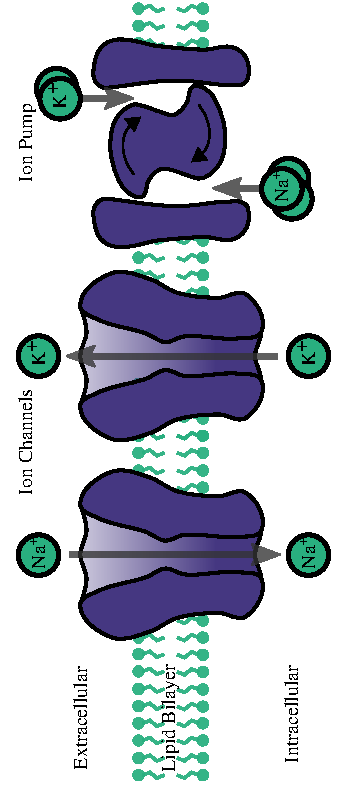
\includegraphics[angle=-90,width=1.0\textwidth]{images/2_1/ion_pumps_0.pdf}
    \caption{Something about ion pumps and channels.}
    \label{fig:2_1_ion_channels}
\end{figure}
The potential difference between the inside and outside the neurons 
are caused by different concentrations of 
ions
in the extracellular and intracellular medium. 
The ions cannot pass through 
the cell membrane as it
consists of a \SI{5}{\nano\metre} lipid bilayer which is mostly impenetrable 
to ions. 

In the membrane sits differnt \emph{ion channels} and 
\emph{ion pumps} which can have selective permeability to ions, this creates 
a potential gradient across the membrane. 
The most significant ions in this process are Sodium (Na$^+$), Potassium (K$^+$), 
Calcium (Ca$^{2+}$), Magnecium (Mg$^{2+}$) and Chloride (Cl$^{-}$). 
Ion channels are divided between passive channels and 
active channels where the active channels can change 
permeability under certain conditions while passive channels have a constant
permeability. 

The ion pumps differ from the channels by activly transporting certain
ions through the membrane. 
For instance, the Sodium-Pottasium exchanger pushes two K$^+$ ions out of the cell
for every three Na$^+$ it pushes into the cell. Doing this creates a net 
loss of charge inside the cell and the pump is therefore electrogenic. 
Not all pumps are electrogenic, the Sodium-Hydrogen exchanger transports
H$^+$ and Na$^+$ without effecting the net charge.
For each H$^+$ ion out of the cell the pump pushes one Na$^+$
into the cell. 

To understand the electrical activity of neurons it is useful
to view the neuron as an electronic circuit where the ion channels, ion pumps
and the membrane serve as different electronic components.

\textcites{hodgkin_quantitative_1952,connor_prediction_1971,sterratt_principles_2011}

% The temperature is important.

%}}} end of Neuronal Models
%{{{ Action Potential
\section{Action Potential}
Action potentials are sharp increases in the membrane potential
followed by a less sharp decrease towards the resting potential. 
In the the depolarization phase the potential rises towards the peak magnitude, 
while in the repolarization phase the potential decreases towards
the cells resting potential.
When the potental is below the resting potential 
it reaches the afterhyperpolarization phase before
it returns to its resting potential.

%}}} end of Action Potential
% Neuron Models {{{ %
\section{Neuron Models}
There are multiple models for neurons, some of the main groups are 
point models and compartmental models. List many models?
Multi-compartmental models 
can be useful to understand the processing of neurons with
complex morphological structures
% }}} 
%{{{ Electrodes
\section{Electrodes}

%}}} end of Electrodes
%{{{ Extracellular
\section{Calculating Extracellular Potential}
The extracellular potential is the electric potential generated from the transmembrane
currents in the neurons. When a neuron fires this can be seen from the extracellular
potential which will have a spike which is similar to the intracellular spike.

By modelling the neuron as
compartments and approximating each compartment as
a spherical volume current source at position $\bf r_0$, the potential at 
at position $\bf r$ at time $t$ will be,
\begin{align}
    {\bf E(r, t)} = \frac{1}{4\pi\sigma}\frac{I_0(t)}{\abs{\bf r - r_0}}
\end{align}

\begin{align}
    {\bf E(r, t)} = \sum^N_{n=1} \frac{1}{4\pi\sigma}\frac{I_n(t)}{\abs{\bf r - r_0}}
\end{align}

Potential from compartments modelled as line sources. 
\begin{align}
    {\bf E(r, t)} &= \frac{1}{4\pi\sigma}\sum^N_{n=1}I_n(t)\frac{dr_n}{\abs{\bf r - r_0}}\\
    &= \frac{1}{4\pi\sigma}\sum^N_{n=1}I_n(t)
        \frac{1}{\Delta s_n}
        \log\abs{\frac{\sqrt{h_n^2 + \rho_n^2} - h_n}{\sqrt{l_n^2 + \rho_n^2} - l_n}}
\end{align}
Taken from \textcite{linden_lfpy:_2013}


This equation rests on two assumptions,
\begin{enumerate}
	\item The permeability $\mu $ of 
	the extracellular medium is the same as that of vacuum $\mu_0$.
	\item The quasistatic approximation which lets the 
	time derivatives, $\partial E/\partial t$, 
	be ignored as source terms.  See \cref{sec:quasi}
\end{enumerate}

The extracellular potential can be calculated
using Maxwell's equations and the continuity equation if the spatial
distribution (morphology) of transmembrane currents and the extracellular conductivity
is known. 



In the quasistatic approximation, since $\nabla\times\bf E = 0$, the
electric field can be expressed with a scalar potential.

Forward problem = calculate the potential from the current source, inverse problem is used
in magnetoenchephalography (important).
The amplitude of a spike in the
extracellular potential is usually in the magnintude of
$< 200 \upmu$V.  
The noise of electrodes vary, but can be as much as $20 \upmu$V. 
This limits the range electrodes can record from. 

The currents sum to zero, while the spike is very visible, there are many small currents
in the dendrites with opposite current. 
(\cite{hamalainen_magnetoencephalography-_1993})

The extracellular spike width tend to increase with distance from soma because of the
neuronal morphology. 
This article used a passive neuron model with different morphologies to show
that the spike width increases with distance to soma. The spike amplitude also
decreases with distance to soma and seems to follow a power law. 
(\cite{pettersen_amplitude_2008} \hspace{-3pt}).

The shape of extracellular spikes are mainly depedent on the membrane currents
and the morphology of the cell. 
Some of the effects from the morphology of the cell are increased spike width and
decreased amplitude from distance to soma. 

Many things here from around page 245. 
When the conductivity $\sigma$ and the current generators are know, Maxwell's
equations and the continuity equation equation can be used to calculate the electric
field $E$ and magnetic field $B$. (TODO: Copied text)
(\cite{hamalainen_magnetoencephalography-_1993})

\subsection*{Background}
% Electric potential from neurons can either be obtained 
% by measuring the membrane potential or measured from the extracellular
% medium. 
%Recording the membrane potential is easier to interpret but harder to execute 
%while 
%extracellular recordings are harder to interpret but easier to execute. 
Recording is usually done using electrodes, this makes recording the membrane potential
more challenging than recording from the extracellular medium as the electrode
has to be very close or inside the cell. 
At the time of writing,
recording the membrane potential of a concious subject is nearly impossible,
this makes understanding extracellular potentials vital for current research. 


Early calculations was done by Rall 1962 investigating 
the interaction between action potentials and synapes using cylinders
as the current source. (TODO: Read article, make more understandble.)
Holt and Koch 1999 added comparmental models to reconstruct pyramidal neurons. 

The information about the transmembrane current is usually difficult to obtain,
as well as the morphology.


%}}} end of Extracellular
%{{{ Neuron and lfpy
\section{Neuron \& LFPy }
LFPy is a Python module that uses Neuron and the mentioned methods to calculate the 
electric field outside the neuron. 
\cite{linden_lfpy:_2013}
\subsection*{Background}

%}}} end of Neuron and lfpy
%{{{ Cell classification

% \section{Cell Type Classification}
% \subsection*{Background}
% It was early observed that the shape of action potentials are different for 
% individual neurons. \textcite{mountcastle_cortical_1969} discovered what
% they called regular spiking and fast spiking.

% \cite{mountcastle_cortical_1969}.

%}}} end of Cell classification
%{{{ Allen Cell Types Database

% \section{Allen Cell Types Database}
% The Allen Brain Institute have gather individual neuron data from lateral geniculate
% nucleus (LGN) and primary visual cortex (V1) of young laboratory mice. 
% The data's main categories are electrophysiology, morphology and modeling.
% With the morphological data the extracellular potential can be calculated given
% a model for the transmembrane currents. 
% % \subsection{Background}

%}}} end of Allen Cell Types Database
%}}} end of Theory
%{{{ Methods
\chapter{Methods}
Methods mentioned here have been developed spesifically for this research. 
\vspace{1em} 
\startcontents
\printcontents{}{1}{\setcounter{tocdepth}{3}}
%{{{ Blue Brain
\section{Blue Brain}
The Blue Brain project released XXX models based upon neurons from 
the hind-limb somatosensory cortex
from 2-week-old Wistar Han rats.
The models were used
The extracellular potential was calculated using 
"TODO: Insert parameters here". 

Use the models. Write code to capture one action potential. Bursting neurons
often hav adapting action potential, what to do there. 

%}}} end of Blue Brain
% Spike Width Measurement {{{ %
\section{Spike Width Measurement}
% TODO: Include sources to different ways of defining spike width.
Many different definitions of spike width has been used to differentiate neurons, but
to date it is not clear which definition is best suited for neuron classification. 
\\

\noindent 
Width Type I - Peak-to-peak: 

Width is measured as the time from the minimum potential to the maximum. 
This is the time from the polarization phase to the afterhyperpolarization phase. 
\newline

\noindent
Width Type II - Width at Half Amplitude:

Width is measured as the duration the spike is below half amplitude of the signal measured
from the baseline at the start of the signal. 
\newline

\noindent
Width Type II - Width at Half Amplitude:

Width is measured as the duration the spike is below half amplitude of the signal measured
from the baseline at the start of the signal. 
\newline

%}}} end of 
% Simulations with LFPyUtil{{{ 
\section{Simulations with LFPyUtil}
LFPyUtil is a python package that was created for this project with the purpose
to simplify the simulation pipeline for multiple neurons and creating
and easy to use interface when developing new simulations. 
LFPyUtil extends and uses the package LFPy to accomplish this. 

The main feature of the python package LFPy is enable the calculation
of extracellular potentials, but another major feature is the simplification
of simulations with the simulation engine Neuron. 
Using Neuron requires a good understanding of the programming language hoc
which creates many challanges as hoc is outdated and is no longer
maintained by the developers. 
To use Neuron with python one has to use the python interface to Neuron
which has been implemented in such a way that runs hoc code directly 
"under the hood". 
A common situation is that one must write hoc code inside strings and
pass them to the python-hoc interpreter. 
This has the unfortunate consequence that the two programming langues are
very intertwined 
and also does not follow
common python coding conventions. 
This also makes it harder for users to troubleshoot errors as problems can
occur either in python, hoc or between the two.
To solve this the package LFPy has attempted to wrap the cell model and
electrodes from the Neuron engine into python objects, such as the 
{\verb LFPy.Cell } and 
{\verb LFPy.StimIntElectrode } classes.

When running a simulation with Neuron there is no inherent support for 
running simulations simultaniously. 
Because LFPy is an extension to Neuron this is also lacking in LFPy. 
LFPyUtil attempts to solve this by starting each simulation
in independent processes. This does not speed up a single simulation
but rather speeds up the simulation of multiple neurons and simulations
that must be run multiple times with different parameters.
The major difficulties of running independent processes with
Neuron is 
that there is no reset function which can make 
the state of the previous simulation effect the state of the next
simulation. 


% TODO: Include sources to the number 0.3 conductivity.
In all simulations the extracellular conductivity was set to 
$\sigma = \SI{0.3}{\ohm\metre}$
based upon data from experimental measurements. 

All stimulus electrodes uses the {\verb LFPy.StimIntElectrode } with 
a custom made electrode named ISyn. With the default stimulus all transmembrane 
currents will be summed
equal the input current, using ISyn prevents this and the currents are correctly
summed to $0$.
\newline

\noindent
The following items are python objects in LFPyUtil.
\newline

SphereRand
\newline
\noindent
SphereRand places
electrodes placed in uniformly distributied locations 
around the soma within a default radius of \SI{50}{\micro\metre}. 
Spike timing is detected by thresholding the soma membrane potential.
That timing is applied to all electrodes such that all electrodes measure
the same part of the simulation. 
If the signal has several spikes
the spike index must be supplied, the default setting uses the first spike.


% }}}
%{{{ Allen Brain Institute
% \section{Allen Brain Institute}

% My spesific implementation of LFPy and Neuron. 

% The recording site for the electrophysiological data is soma for all neuron in the data from 
% Allen Brain Institute.
% The currents in the dendrites are not avaiable and is modelled using a passive neuron model.
% Write how the simulation is set up. 


% Create convincing results that shows that the simulations are correct and can be trusted. 

% \begin{itemize}
% 	\item Action potential width and amplitude is correct. 
% 	\item Fourier specter is correct. 
% 	\item Extracellular width and amplitude matches the article. 
% 	\item Create same plots. 
% 	\item Calculate the same parameters, power law?
% \end{itemize}

% How different are action potentials generated from the same cell. How does the "mean" spike look
% from the experimental data. 

% Data from Blue Brain and Allen Brain Institute. 

% Allen Brain Institute Questions:
% \begin{itemize}
% 	\item How much does the experimental spikes differ. 
% \end{itemize}

%}}} end of Allen Brain Institute
%}}} end of Methods
%{{{ Results
\chapter{Results}
In figure ?? the spike width from interneurons and pyramidal neurons have been
plottet seperatly. Neurons in the pyramidal group are the type TTPC1 and TTPC2 
The groups suggests that interneuron can be seperated from 
pyramidal neurons depending on their spike shape. 

\vspace{1em} 
\startcontents
\printcontents{}{1}{\setcounter{tocdepth}{3}}

%{{{ Pettersen and Einvoll
\section{Pettersen \& Einevoll (2008) Reproduction}
To verify that the simulation environment could be trusted 
some results from 
\textcite{pettersen_amplitude_2008} was replicated.
Spesifically the spike width and amplitude dependency in relation to 
the distance from soma was compared to current results. 

% Write more about the connor stevens model?

\subsection{Simulation}
\emph{Cell:}
The \textcite{mainen_influence_1996} cell was used with a passive model, which is 
the same model used in \textcite{pettersen_amplitude_2008}. 
It is not clear in which plane the measurements was taken from so 
the cell was rotated using PCA (principal component analysis) on the compartment
positions.
This rotates the cell so most of the dendrites are along
the y and x-axis. 
\\
% TODO: show the morphology of the neuron

\noindent\emph{Spike Generation:}
An action potental was generated using the Connor-Stevens model 
\cites{connor_prediction_1971, connor_neural_1977}
using the same parameters as \textcite{dayan_theoretical_2001}. 
This had an amplitude of $107.6mV$ from baseline with the peak at $48.21mV$. 
These values are similar (TODO: how similar?) to \textcite{dayan_theoretical_2001}, but not
with \textcite{pettersen_amplitude_2008} which had an amplitude of 
$83mV$ from baseline. To compensate for the difference the action potental was 
normalized to $83mV$ manually (\cref{fig:3_1_soma_mem}).
\\

\begin{figure}[h]
\centering
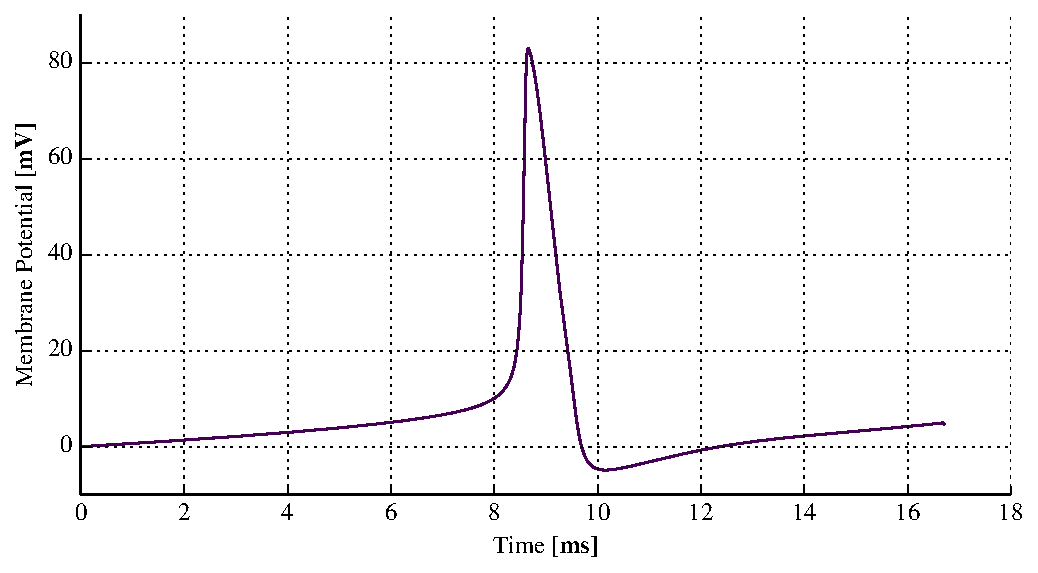
\includegraphics[width=1\textwidth]{images/3_methods/3_1_reproduction/soma_mem.pdf}
\caption{Soma membrane voltage. }
\label{fig:3_1_soma_mem}
\end{figure}


\noindent\emph{Parameters:}
Parameters are the same as \textcite{pettersen_amplitude_2008} and 
\textcite{dayan_theoretical_2001} . Membrane resistance 
$R_m = 3\cdot10^4\Omega /cm^2$, membrane capacitance $C_m=1\mu F / cm^2$, 
axial resistance $R_a = 150\Omega/cm^2$, time resolution $dt=2^{-6}ms$. 
The reversal potential was set to zero. The action potental was imposed in all
soma sections using the "play" vector function in Neuron.
\\

\noindent\emph{Electrode Positions:}
Recording sites were placed in the xz plane at 11 linearly spaced 
positions along 36 lines with equal 
angular spacing. (TODO: Show the electrode positions.) 
\\


\noindent\emph{Spike Width \& Amplitude:}
A baseline was set as the value at the start of the signal. 
Amplitude was calculated as the difference between maximum absolute value and the
baseline.
The spike width was calculated at half width at maximum amplitude. 

Spike width was recorded at $0.5625 ms$ for $dt=2\cdot10^{-5}$, similar to 
$0.55ms$ from \textcite{pettersen_amplitude_2008}. When increasing the
resolution to $dt=2\cdot10^{-6}ms$ the spike width rose to $0.625ms$. 


\subsection{Results}
The action potental that was used in \textcite{pettersen_amplitude_2008} 
is similar to the one used here.  The amplitude of the fourier transform is displayed in
\cref{fig:3_1_fourier}, which is in close resemblance to the standard action potential
in Fig. $3$ in the paper. 

\begin{figure}[thp]
\centering
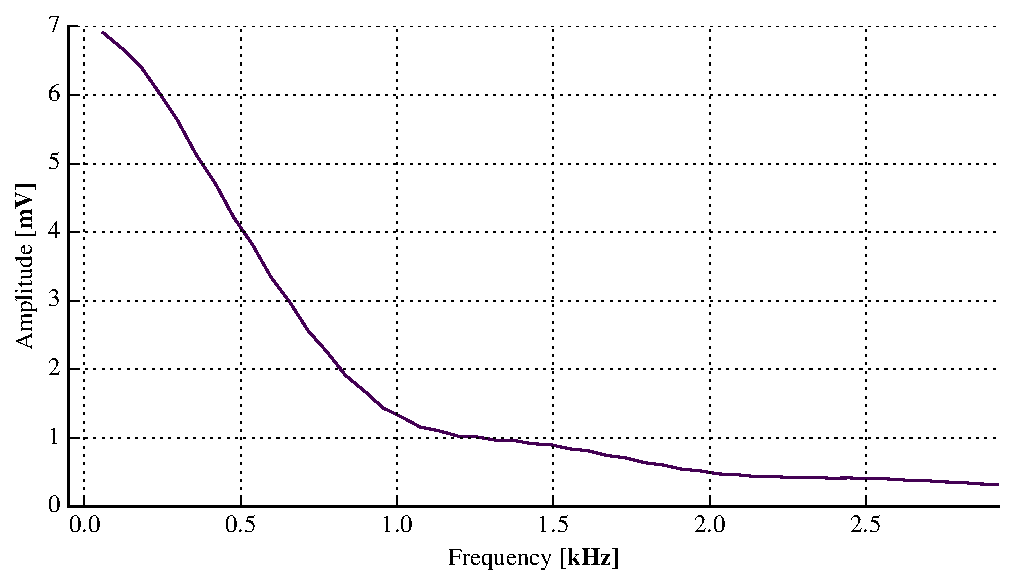
\includegraphics[width=\textwidth]{images/3_methods/3_1_reproduction/soma_mem_fourier.pdf}
\caption{Frequency specter of simulated somatic membrane potential.}
\label{fig:3_1_fourier}
\end{figure}

The spike width increases with the distance from soma as seen in 
\cref{fig:3_1_spike_width}. These results are 
lower than the widths reported in \textcite{pettersen_amplitude_2008}.
(Use more time on editing the Connor-Stevens model to come closer to 
an max.amplitude on 20mV?).   

Sudden changes in spike width was experienced with increased distance from
soma. Above $200\mu V$ the
spikes shapes are not well defined. 
This was also reported in \textcite{pettersen_amplitude_2008}.\\

\begin{figure}[thp]
\centering
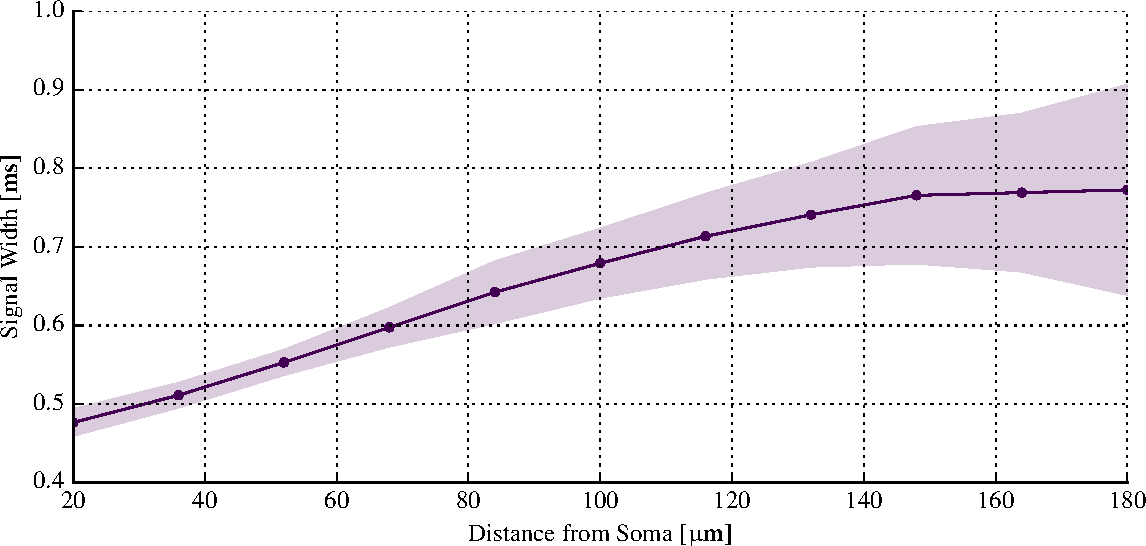
\includegraphics[width=\textwidth]{images/3_methods/3_1_reproduction/circular_spike_width_std.pdf}
\caption{Spike width over distance. Mean +/- 1 std.}
\label{fig:3_1_spike_width}
\end{figure}

\textcite{pettersen_amplitude_2008} reports a spike amplitude above $150\mu V$ at 
$20\mu m$, this does not match current findings.  
\cref{fig:3_1_spike_amp} shows spike amplitude with logarithmic axes.  
(TODO: Is numbers on the power law decays necessaryy?) Although 
the data does not match \textcite{pettersen_amplitude_2008}, 
it is comparable with what is
expected in the near and far limit field of a ball and stick neuron.
In the near field the the expectation is a $1/r$ decay and in the far field
it is  $1/r^2$ or $1/r^3$ depending on distance. (TODO: Clearify this, put reference
back to theory chapter.)

\begin{figure}[thp]
\centering
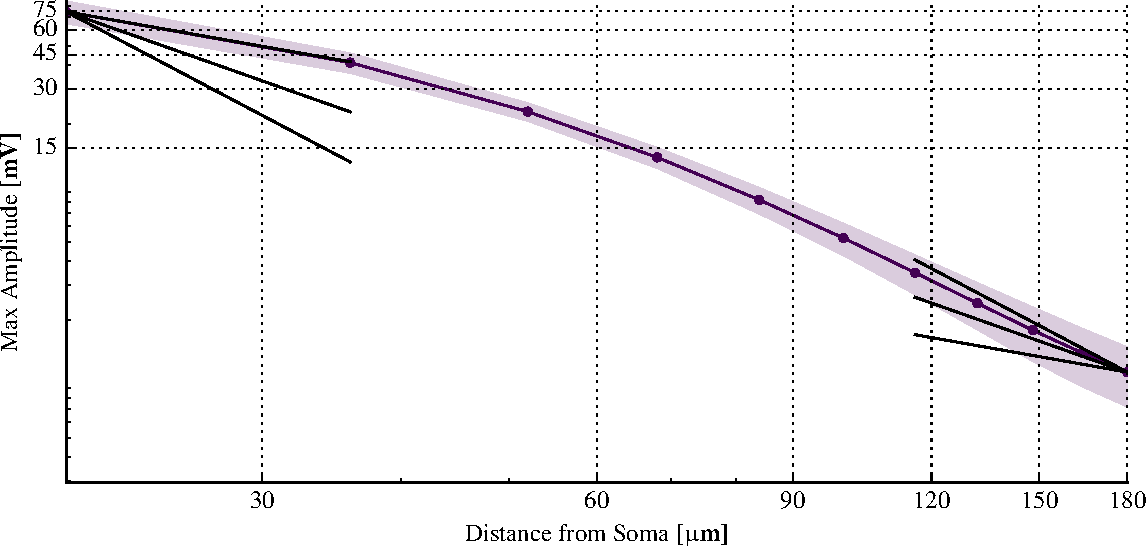
\includegraphics[width=\textwidth]{images/3_methods/3_1_reproduction/circular_spike_amp_std_log.pdf}
\caption{Spike amplitude over distance. Mean +/- 1 std. The power law
decays $1/r$, $1/r^2$ and $1/r^3$ are shown at the leftmost and rightmost
data points.}
\label{fig:3_1_spike_amp}
\end{figure}

\subsection{Discussion}

%}}} end of Pettersen and Einvoll

%}}} end of Results
%{{{ Discussion
\chapter{Discussion}
Nothing here yet.


%}}} end of Discussion
%{{{ Appendix
% \begin{appendix}
% \chapter{Appendix}
% \section{Quasistatic Approximation in Neural Tissue}
% \label{sec:quasi}
% A quasistatic approximation implies that the equations have a form that does
% not include time derivatives (static). Some quantaties can be allowed to vary over 
% time, but slowly. 
% 	Here we show that the quasistatic approximation is a valid assumption in
% neural tissue. First start with Maxwell's equations.
% \begin{align}
% 	\nabla \cdot {\bf E} &= p / e \nonumber\\
% 	\nabla \times {\bf E} &= -\partial \bf{B} / \partial t \label{eq:max_1}\\
% 	\nabla \cdot {\bf B} &= 0\nonumber\\
% 	\nabla \times {\bf B} &= \mu_0({\bf J} + \epsilon_0\partial{\bf E}/\partial t)
% 	\label{eq:max_3}
% \end{align}

% In a passive nonmagnetic medium, {\bf J} is the sum of ohmic volume current 
% and the polarization current
% \begin{align}
% 	\bf J &= \sigma{\bf E} + \partial {\bf P}/\partial t \label{eq:cur_den_0}
% \end{align}
% where ${\bf P} = (\epsilon - \epsilon_0){\bf E}$ is the polarization and $\epsilon$
% is the permitivity of the material.In neuromagnetism, we generally deal with
% frequencies that are below 100 \si{\hertz}. Cellular electrical
% phenomena contain mostly frequencies below \si{1\kilo\hertz}. 
% Let $\sigma$ and $\epsilon$ be uniform and let us consider elctromagnetic 
% wave at frequencty $f$.
% \begin{align}
% 	{\bf E} = {\bf E}_0({\bf r})\exp(i2\pi ft)
% \end{align}
% With \cref{eq:max_3,eq:cur_den_0} we get,
% \begin{align}
% 	\nabla \times {\bf B} &= \mu_0(
% 		\sigma{\bf E} + 
% 		(\epsilon - \epsilon_0)\partial{\bf E}/\partial t + 
% 		\epsilon_0\partial{\bf E}/\partial t
% 		)
% \end{align}
% For the quasistatic approximation to be valid, it is necessary
% that the time-derivative terms be small compared to the 
% ohmic current. 
% \begin{align}
% 	\abs{\epsilon{\bf E}/\partial t} \ll \abs{\bf \sigma E} 
% 		\rightarrow 2\pi f \epsilon/\sigma \ll 1
% \end{align}
% With $\sigma = 0.3\,\si{\per\ohm\per\meter}$, the value of brain tissue, 
% $\epsilon = 10^5\cdot\epsilon_0$, and $f = 100\,\si{\hertz}$, we find
% \begin{align}
% 	2\pi f\epsilon/\sigma = 2\cdot10^{-3} \ll 1
% \end{align}
% In addition, $\partial {\bf B} /\partial t$ must be small. from
% \cref{eq:max_1,eq:max_3}, 
% \begin{align}
% 	\nabla\times\nabla\times{\bf E} &= 
% 		-\frac{\partial}{\partial t}(\nabla\times{\bf B})\nonumber\\
% 	&= -\mu_0\frac{\partial}{\partial t}
% 		(
% 		\sigma{\bf E} + \epsilon\partial{\bf E}/\partial t
% 		) \nonumber \\
% 	&= -i2\pi f\mu_0(\sigma + i2\pi f\epsilon){\bf E}
% \end{align}

% Solutions of this equation have spatial changes on the characteristic
% length scale
% \begin{align}
% 	\lambda_c = \abs{2\pi f \mu_0 \sigma(1+i2\pi f \epsilon/\sigma)}^{-1/2}
% 		\approx65\,\si{\meter}
% \end{align}
% This length is much longer than the diameter of the head. This implies that the
% contribution of $\partial {\bf B}/\partial t$ to $\bf E$ is small. Theautorefor,
% the quaasistatic approximation appears justified. This does not
% mean that we should forget time-dependent phenomena altogether. 
% For example, the capacitative current through the cell membrane is significant in
% determining the properties of the action potential. 
% Nevertheless, this so-called displacement current, 
% $\epsilon_0\partial{\bf E}/\partial t$, need not be taken into account in the 
% calculation of $\bf B$.

% Copied from
% \textcite{hamalainen_magnetoencephalography-_1993}

% \end{appendix}
%}}} end of Appendix
%{{{ Glossary
% \printglossary[style=mcoltreegroup]
%}}} end of Glossary
%{{{ Bibliography
%\nocite{*}
\printbibliography[heading=bibintoc]
%}}} end of Bibliography
\end{document}
